\biohead{Moses Hezelwood}{}

Moses Hezelwood was born on 23 March 1777 in 	Ruswarp, Yorkshire to Thomas Hezelwood (\p{Thomas_Hezelwood}) and Mary (unknown)(\p{Mary_Unknown}) and christened on 15 June 1777 in	Whitby, Yorkshire, England.\cite{MHezelwoodBirth} He had four siblings: Thomas Hezelwood (1766--1781), Hannah Hezelwood (b.21 May 1768), John Hezelwood (b.7 August 1774) and Aaron Hezelwood (b.30 May 1779).

He married Elizabeth Mead (\p{Elizabeth_Mead}) on 22 April 1802 in	Whitby, Yorkshire.\cite{MHezelwoodMarriage}  They had eight children: Mary Hezelwood (1805--1887), Elizabeth Hazelwood (\p{Elizabeth_Hezelwood}), Isabella Hazelwood (1808--1882), Sarah Hazelwood (1811--?), Francis Medd Hazelwood (1813--), Thomas Hezelwood (1813/4--1851), Francis Hazelwood (1816--?) and Trufit Mead Hazelwood (1817--?). (According to notes made by his grandson, Thomas Henry Barker, Moses  was of ``old Yorkshire parentage, probably of the family of Hesslewood (Danes) superceded by the Vavasours.'' Also according to these notes, he and Elizabeth had 17 children, of whom only 4 reached maturity: but this is unverified.)

\begin{figure}
 \centering
 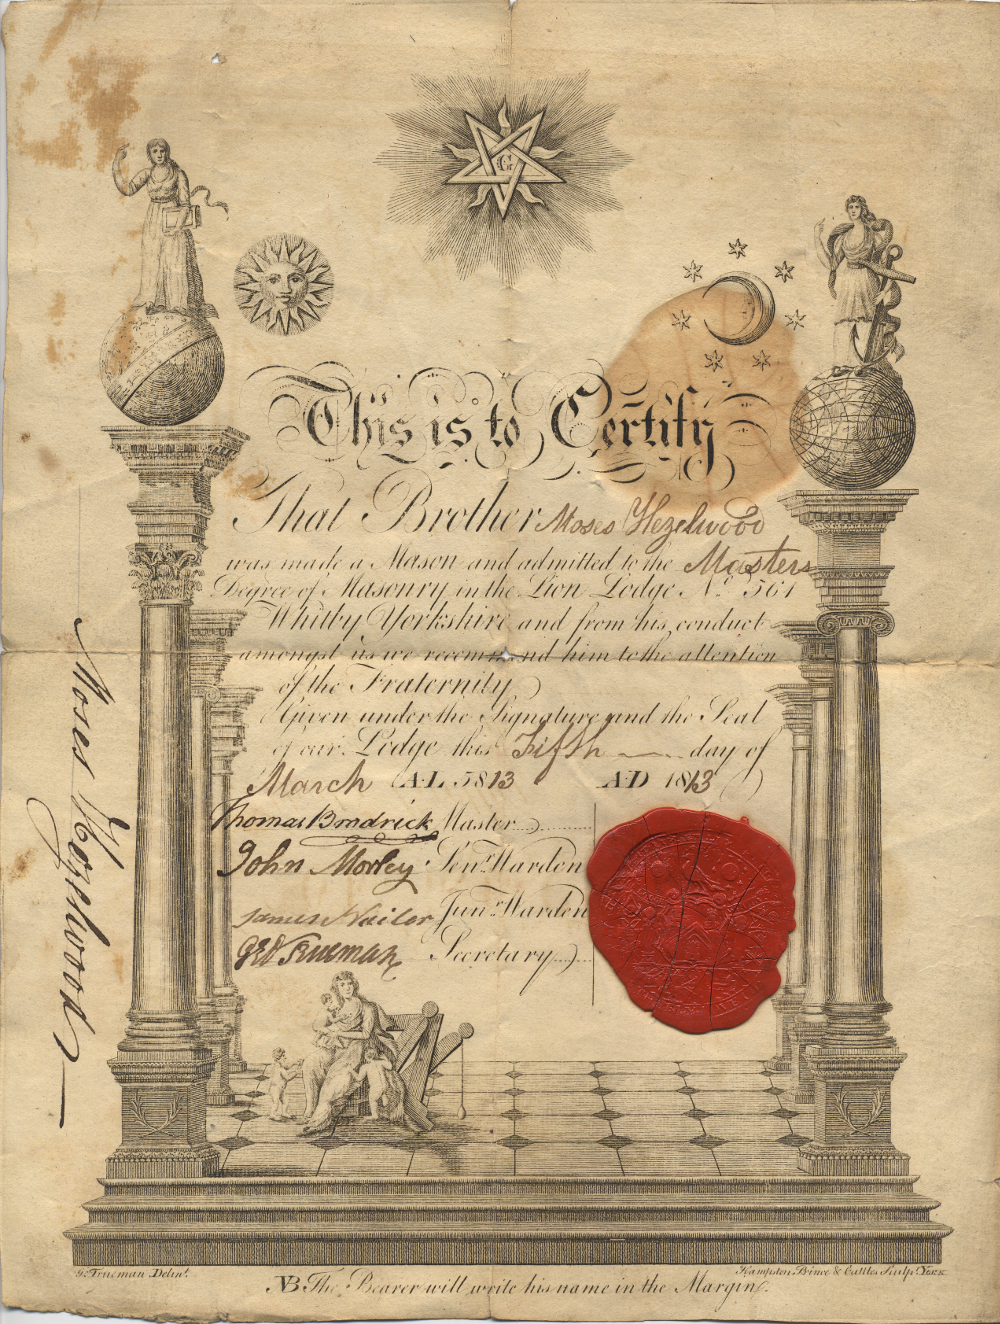
\includegraphics{sources/MosesHezelwoord_MasonicCert_1813.png}
 \caption{Certificate of Masonic brotherhood, March 1813.}
\end{figure}

In 1841 he was living in Bathgate, Whitby \cite{MHezelwood1841} and by 1851 he was a lodger at 7 Flowergate, Whitby, Yorkshire and he was employed as a Cabinetmaker and Mason.\cite{MHezelwood1851}

It seems that at one point in his life he was bankrupt: the following is taken from the London Gazette, 1854:\cite{MHazelwoodBankruptcy}

\begin{quotation}
\textsc{Whereas} the Assignees of the estate and effects of Moses Hezelwood, late of Whitby, in the North Riding of Yorkshire, Cabinet-Maker, an `Insolvent Debtor, lately a Prisoner' in the Gaol of York Castle, in the County of York, have caused their account of the said estate and effects, duly sworn to, to be filed in the Court for Relief of Insolvent Debtors; the Creditors of the said Insolvent are requested to meet the Assignees at the House of Mr. Jonathan Featherstone, the Swan Inn, in Whitby aforesaid, on the 14th day of November next, at Two of the Clock in the Af- ternoon precisely, when and where the Assignees will declare the amount of the balance in their hands, and proceed to make a Dividend with the same amongst the Creditors whose debts are admitted in the schedule sworn to by the Insolvent, in proportion to the amount thereof, subject to such correction of the rights to receive dividends as may be made according to the Statute. If any person Has a demand which is Stated in the schedule, but is disputed therein, either in whole or in part; or if the said Insolvent, the said Assig. nees, or any Creditor, object to any debt mentioned thereif, such claims and objections must be brought forward at the said meeting, in order that proceedings may be had for the examination and decision of the same according to the Statute.
\end{quotation}

By 1861 he was retired and living in Bagdale, just outside Whitby. \cite{MHezelwood1861}

Moses died on 14 February 1868 in Whitby, Yorkshire, and was buried on 18 February 1868 in Sneaton Churchyard,	Whitby, Yorkshire: \cite{MHezelwoodDeath} and a note made by his daughter Elizabeth reads: ``Dear Father died on the 14th February 1868 at Whitby in his ninety-first year.''

An obituary piece in the Whitby Gazette read as follows:
The Late Mr. Moses Hezelwood:
In consequence of an incorrect notice of our late venerable townsman having appeared in a contemporary, we are requested to insert in our columns the following brief but well authenticated account.
"Recently, we had to record the death of our long esteemed fellow townsman, Mr. Moses Hezelwood, at the very advanced age of 90 years. Mr. Hezelwood was amongst the first of our tradesmen at the opening of the present century, when he carried on the business of cabinet maker on the premises at the foot of Golden Lion Bank. He was a man of unflinching temperament, whether in trade, patriotism, or amusement, and as active and athletic as any of his contemporaries. Taking a great interest at all times in movements of a political character, he caused himself to be enrolled a volunteer, when the movement in 1803 first originated the body. HIs aptitude for drill and manly bearing soon won for him a Sergeantcy. His interest and exertions in governmental elections, even up to the very last, was most noticeable. In 1812 he became a master mason, as his certificate now before us shows, and at the time of his death was the oldest in the town, and the oldest of the Lodge to which he belonged, excepting perhaps, one member, now a non-resident. As a walker and follower of the piscatory art, too, he was unrivalled int the district, having accomplished, in respect to the first, 70 miles in a single day. As a fisherman, rising before the dawn, he was to be met by the beckside, or wading up to his middle in the Esk, and seldom failed to secure both b y his diligence and expertness in casting the fly, a basket of fish. Some years ago he retired from business, and spent the remainder of his days in a house in Bagdale. As an illustration of his longevity, and to show how long such lives seem to us by comparison, we may say that he was 38 years of age when Waterloo was fought; that he enjoyed a married life of 32 years, and has been 32 years a widower. In conclusion, we may just say, that he was carried to his last resting place in Sneaton Church-yard, on Thursday the 20th ult., his remains attended by two surviving daughters and many townsmen and brother masons who recognized his worth. Finally, we may remark in contrast to Longfellow's idea, 'Lives of great men all remind us, we can make our lives sublime,' that lives of such men also show us, how, without the qualification of greatness, me may spend our days honourably, actively, and usefully." \cite{MHezelwoodDeathnotice}
